\documentclass[12]{article}%12pt即为*四号字
\usepackage{ctex}%引入中文包
\usepackage{graphicx}%插入图片的包
\usepackage{geometry}%设置A4纸页边距的包
\usepackage{url}
\usepackage{stfloats}
\usepackage{float}

\geometry{left=3.18cm,right=3.18cm,top=2.54cm,bottom=2.54cm}%设置页边距
\linespread{1}%设置行间距



\begin{document}
\begin{center}
    \LARGE\songti\textbf{Chapter 4 Programming Assignments} \\%标题
    \large\kaishu\textbf{褚朱钇恒\qquad 3200104144}%一般是我的姓名
\end{center}
    \section{Programming Assignments}
        \subsection{A}
            The values of the functions in (4.49) at 101 equally spaced points covering the interval [0.99, 1.01] is in the file $A.out$ in folder $data$.There are the values plot on the axis.
        \begin{figure}[H]
            \centering
            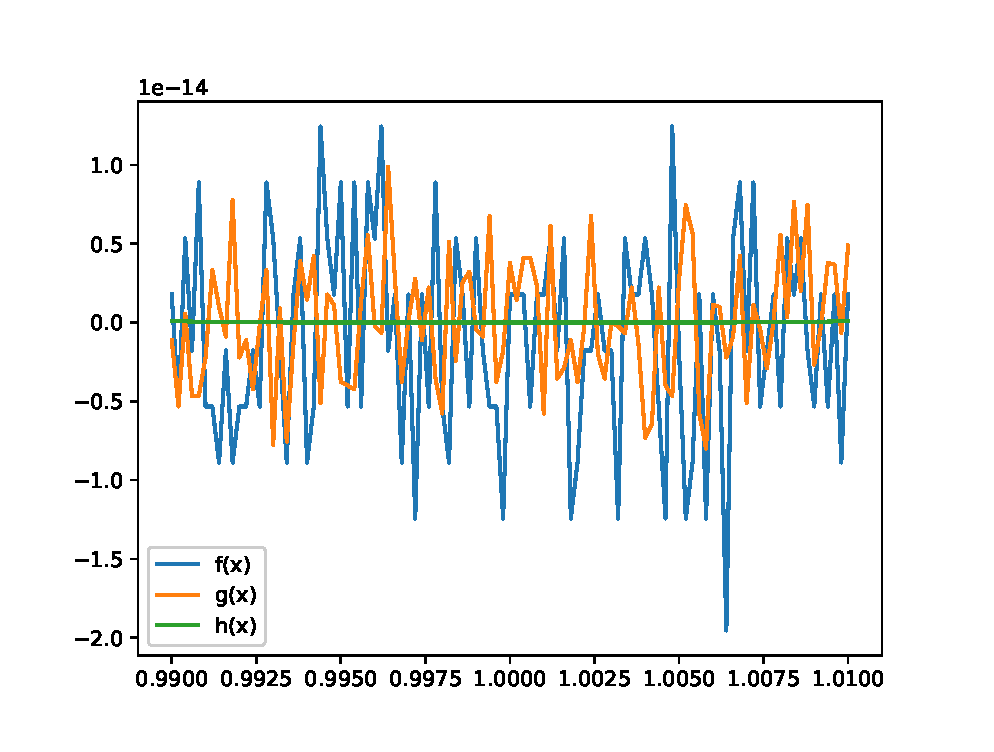
\includegraphics[width=0.7\textwidth]{./pic/A.eps}
            \caption{Values of f, g and h on [0.99, 1.01]}
        \end{figure}

        It's obvious that the blue line has the largest vibration amplitude on the interval. It means this algorithm is very unstable when trying to find the exact value of the function. The reason may be that the maximum number of calculations is used and a large rounding error is introduced.

        The yellow line has less calculation times, so the rounding error is small, the curve vibration amplitude is small, and the result is more accurate.

        The algorithm corresponding to the green line has the least number of operations and the most accurate result.
        \subsection{B}
            From definition, we get $OFL=0.5,UFL=3.5$

            There are 25 numbers in this normalized FPN system, they are:

            -3.5 -3 -2.5 -2 -1.75 -1.5 -1.25 -1 -0.875 -0.75 -0.625 -0.5 0 0.5 0.625 0.75 0.875 1 1.25 1.5 1.75 2 2.5 3 3.5
            
            This is the normalized FPN system's image on the real axis.
            \begin{figure}[H]
                \centering
                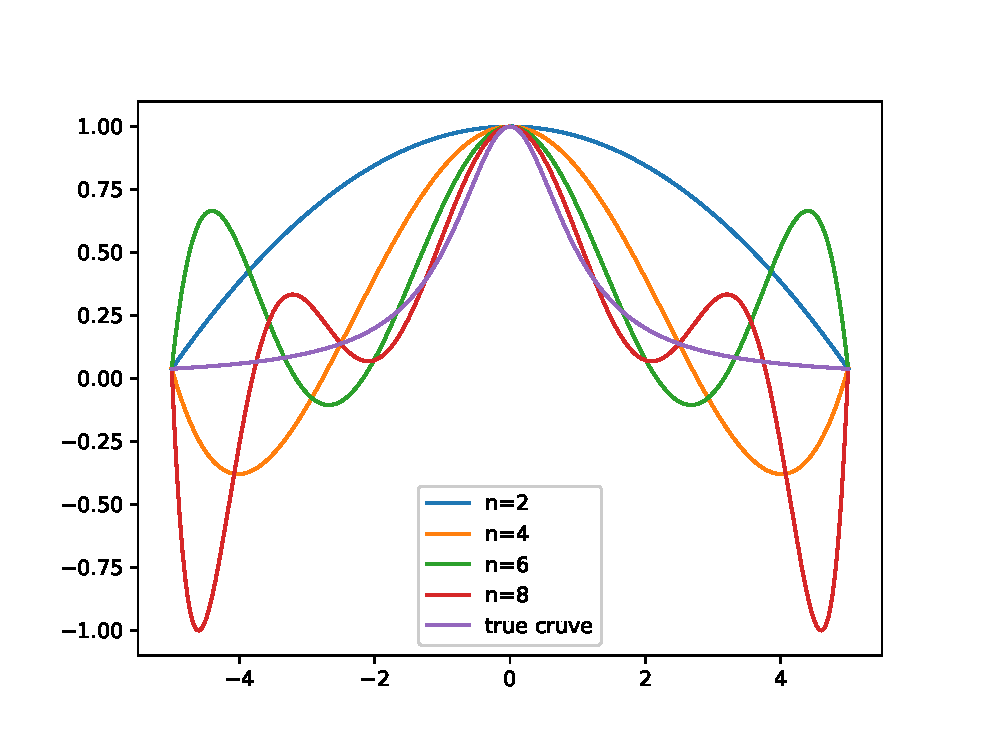
\includegraphics[width=0.7\textwidth]{./pic/B.eps}
                \caption{normalized FPN}
            \end{figure}

            There are 6 numbers in this subnormal FPN system, they are:

            -0.375 -0.25 -0.125 0.125 0.25 0.375 

            This is the subnormal FPN system's image on the real axis.
            \begin{figure}[H]
                \centering
                \includegraphics[width=0.7\textwidth]{./pic/sB.eps}
                \caption{subnormal FPN}
            \end{figure}
\end{document}